\documentclass[12pt]{article}
\usepackage{ctex}
\usepackage[english]{babel}
\usepackage{blindtext}
\usepackage{nameref}
\usepackage{fancyhdr}
\usepackage{amsmath,amssymb,amsthm}
\usepackage{graphicx,float}
\usepackage{physics}
\usepackage{pgfplots}
\usepackage[a4paper, total={7in, 9in}]{geometry}

\graphicspath{{./img/}}

\pagestyle{fancy}
\fancyhf{}
\fancyhf[HL]{測驗1:二項式定理、指數及對數}
\fancyhf[CF]{\thepage}

\newcommand{\innerprod}[2]{\langle{#1},{#2}\rangle}
\newcommand{\id}{\mathtt{id}}

\newtheorem{definition}{定義}
\newtheorem*{theorem}{定理}
\newtheorem*{corollary}{衍理}
\newtheorem*{lemma}{引理}
\newtheorem*{proposition}{設理}
\newtheorem*{remark}{小記}
\newtheorem*{claim}{主張}
\newtheorem*{example}{例子}
\newtheorem*{axiom}{公設}
\renewenvironment*{proof}{\textit{證明.}}{\hfill$\qed$}

\newenvironment*{sol}{\par \textbf{解}.}{\hfill$\blacksquare$}

\begin{document}
    \thispagestyle{empty}

    \centering 

    \section*{測驗1\\數學延伸單元\\單元1 (微積分與統計學)\\試題-答題簿}

    限時: 1 小時

    姓名:\hrulefill \hfill 得分:\hrulefill/20

    學校:\hrulefill

    \raggedright

    \subsection*{規則}

    \begin{enumerate}
        \item 此試卷必須使用中文回答。
        \item 除特別指明外,需詳細列出所有算式。
        \item 除特別指明外,數值答案必須用真確值表示。
        \item 本試卷只作\textbf{内部使用}。
        \item 所有試題取自AL/CE/DSE歷届試題,來源: https://www.dse.life/ppindex/m2/
    \end{enumerate}
    \newpage
    \thispagestyle{empty}
    \vspace*{\fill}
    \begin{center}
        -此爲空白頁-
    \end{center}
    \vspace*{\fill}
    \newpage
    \setcounter{page}{1}
    \begin{enumerate}
        \item (5分)\begin{enumerate}
            \item 依$u$的降冪次序展開$(u+\frac{1}{u})^4$。
            \item 依$x$的升冪次序展開$(e^{ax}+e^{-ax})^4$至含$x^2$的項爲止。
            \item 假設在(b)題的結果中$x^2$的係數為2,求$a$的所有可能值。
        \end{enumerate}

        \hrulefill

        \hrulefill

        \hrulefill

        \hrulefill

        \hrulefill

        \hrulefill

        \hrulefill

        \hrulefill

        \hrulefill

        \hrulefill

        \hrulefill

        \hrulefill

        \hrulefill

        \hrulefill

        \hrulefill

        \hrulefill

        \hrulefill

        \hrulefill

        \hrulefill

        \hrulefill

        \hrulefill

        \hrulefill

        \hrulefill

        \hrulefill
        \item (6分)\begin{enumerate}
            \item 依$x$的升冪次序展開$(1+e^{3x})^2$至含$x^2$的項爲止。
            \item 求$(5-x)^4(1+e^{3x})^2$的展開式中$x^2$的係數的值。
        \end{enumerate}

        \hrulefill

        \hrulefill

        \hrulefill

        \hrulefill

        \hrulefill

        \hrulefill

        \hrulefill

        \hrulefill

        \hrulefill

        \hrulefill

        \hrulefill

        \hrulefill

        \hrulefill

        \hrulefill

        \hrulefill

        \hrulefill

        \hrulefill

        \hrulefill

        \hrulefill

        \hrulefill

        \hrulefill

        \hrulefill

        \hrulefill

        \hrulefill
        \item (6分)已知池塘裏受某個疾病影響的魚的數量$N(t)$能以下式模擬:$$N(t)=\frac{500}{1+ae^{-kt}}$$其中$a,k$為正常數,而$t$為由疾病發生起所經歷的日數。
        \begin{center}
            \begin{tabular}{|c|c|c|c|c|}
                \hline
                $t$&5&10&15&20\\
                \hline
                $N(t)$&13&34&83&175\\
                \hline
            \end{tabular}
        \end{center}
        \begin{enumerate}
            \item 將$\displaystyle\ln\biggl(\frac{500}{N(t)}-1\biggr)$表為$t$的線性函數。
            \item 利用以下圖表,估算$a$和$k$的值。(請將答案取值至小數點後一個位)\begin{figure}[H]
                \centering
                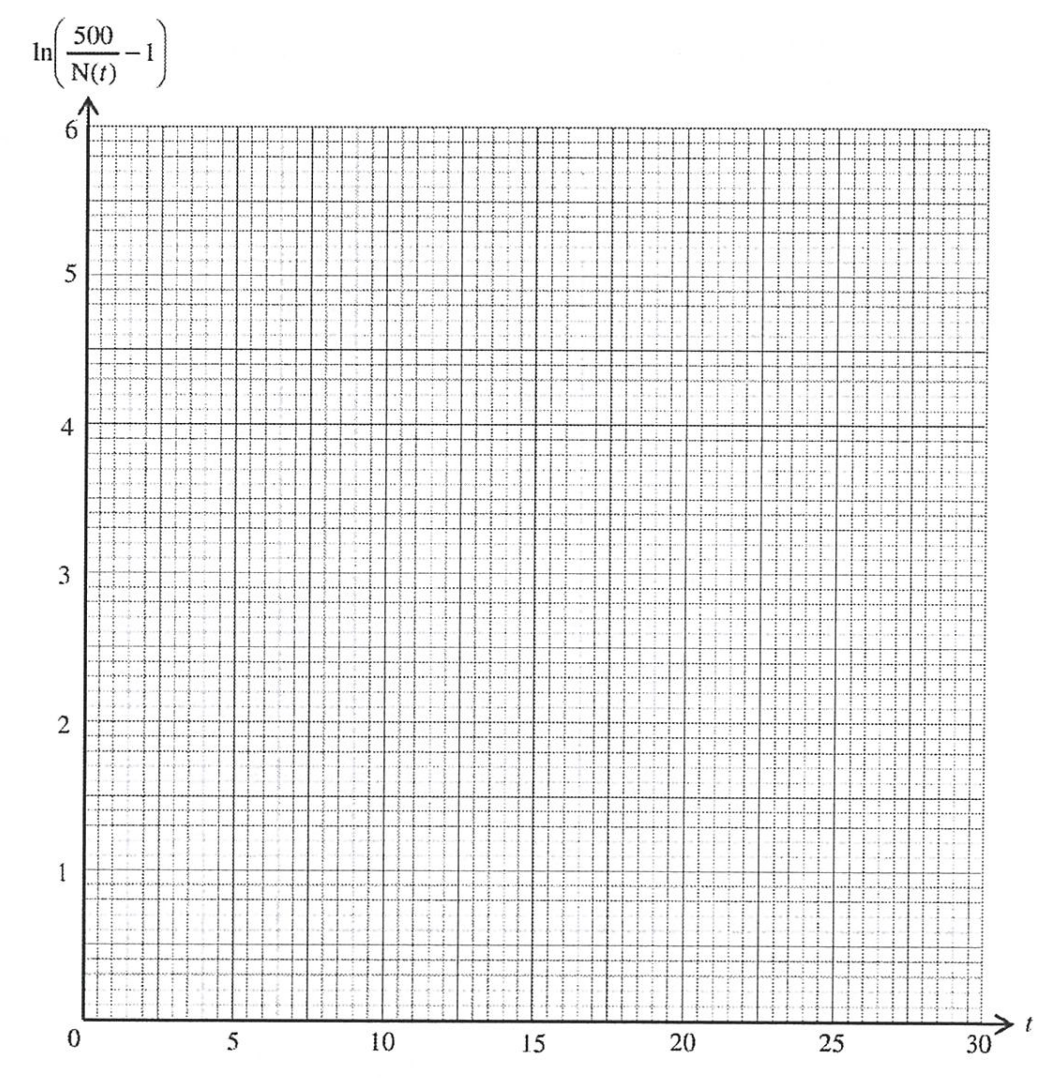
\includegraphics[scale=0.75]{graph_paper.png}
            \end{figure}
            \item 請問受感染的魚的數量將在疾病爆發後的多少天到達270條?
        \end{enumerate}

        \hrulefill

        \hrulefill

        \hrulefill

        \hrulefill

        \hrulefill

        \hrulefill

        \hrulefill

        \hrulefill

        \hrulefill

        \hrulefill

        \hrulefill

        \hrulefill

        \hrulefill

        \hrulefill

        \hrulefill

        \hrulefill

        \hrulefill

        \hrulefill

        \hrulefill

        \hrulefill

        \hrulefill

        \hrulefill

        \hrulefill

        \hrulefill

        \hrulefill

        \hrulefill

        \hrulefill

        \hrulefill

        \hrulefill

        \hrulefill

        \hrulefill

        \hrulefill

        \hrulefill

        \hrulefill

        \hrulefill

        \hrulefill

        \hrulefill

        \hrulefill

        \hrulefill

        \hrulefill

        \hrulefill

        \hrulefill

        \hrulefill

        \hrulefill

        \hrulefill

        \hrulefill

        \hrulefill

        \hrulefill

        \hrulefill

        \hrulefill

        \hrulefill

        \hrulefill

        \hrulefill

        \hrulefill

        \hrulefill

        \hrulefill
        \item[挑戰題.] (4分)設$p$為實數且$0<p<1$。設$n$為正整數。對$k$介乎$1$與$n$之間,定義$a_k=C_k^n p^k(1-p)^{n-k}$。\begin{enumerate}
            \item 證明$\displaystyle\sum_{k=0}^{n}a_k=1$。
            \item 證明$k\cdot C_k^n=n\cdot C_{k-1}^{n-1}$。由此證明$\displaystyle\sum_{k=0}^{n}ka_k=np$。
        \end{enumerate}

        \hrulefill

        \hrulefill

        \hrulefill

        \hrulefill

        \hrulefill

        \hrulefill

        \hrulefill

        \hrulefill

        \hrulefill

        \hrulefill

        \hrulefill

        \hrulefill

        \hrulefill

        \hrulefill

        \hrulefill

        \hrulefill

        \hrulefill

        \hrulefill

        \hrulefill

        \hrulefill

        \hrulefill

        \hrulefill

        \hrulefill

        \hrulefill

        \hrulefill

        \hrulefill

        \hrulefill

        \hrulefill

        \hrulefill

        \hrulefill

        \hrulefill

        \hrulefill

        \hrulefill

        \hrulefill

        \hrulefill

        \hrulefill

        \hrulefill

        \hrulefill

        \hrulefill

        \hrulefill

        \hrulefill

        \hrulefill

        \hrulefill

        \hrulefill

        \hrulefill

        \hrulefill

        \hrulefill

        \hrulefill

        \hrulefill

        \begin{center}
            -全卷完-
        \end{center}
    \end{enumerate}
\end{document}